\input{\InDir/All.tex/outcomes-macros-def}
\input{\InTexDir/outcomes-macros}
\input{\InDir/All.tex/expand-outcomes}
 
\input{\InTexDir/firstpage}				\newpage
\input{\InTexDir/copyright}				\newpage
 
\pagenumbering{roman}
\setcounter{page}{1}
\pagestyle{plain}
\input{\OutputTexDir/team-ES}					\newpage 
\input{\InTexDir/abstract}	\newpage
 
\tableofcontents
\listoffigures
\listoftables
  
\input{\InProgramDir/ack}			\newpage
\input{\OutputTexDir/acronyms}		\newpage
. \newpage
 
\begin{btUnit}
\pagestyle{plain}
\pagenumbering{arabic}
\setcounter{page}{1}

%\OnlySPC{\input{\InTexDir/about-this-document}}
%\input{\InTexDir/chap-introduction}

% % %\part{Otra parte}
%\input{\InTexDir/BodyOfKnowledge}

%%%%%%%%%%%%%%%%%%%%%%%%%%%%%%%%%%%%%%%%%%%%%%%%%%%%%%%%%%%%%%%%%%%%%%%%%%%%%%%%%%%%%%%%%%%%%%%
% Malla, outcomes/course, KU by course, etc
% \input{\InTexDir/GeneralInfo}
\chapter{Plan de estudios \YYYY}\label{chap:GeneralInfo} 

\section{Clasificación de los cursos por niveles}
De acuerdo a la \textit{Computing Curricula}, los cursos son clasificados en 3 niveles: Introductorios (Códigos 100), 
Intermedios  (Códigos 2..), Avanzados  (Códigos 3..) y orientados a la construcción del trabajo de final de carrera  (Códigos 4..) también llamado tesis.

Los cursos de tercer nivel tienen por objetivo abrir varias posibilidades de especialización a través de cursos electivos

Esta propuesta de malla curricular está basada en el abordaje orientado a objetos. 
El abordaje orientado a la web se escogió porque hacia eso apuntan las tendencias 
futuras de la computación.

\section{Codificación de los cursos}
Los cursos se encuentran codificados bajo el esquema que se muestra en la Figura~\ref{fig:course-coding}:

\begin{latexonly}
      \begin{figure}[ht]
      \centering
      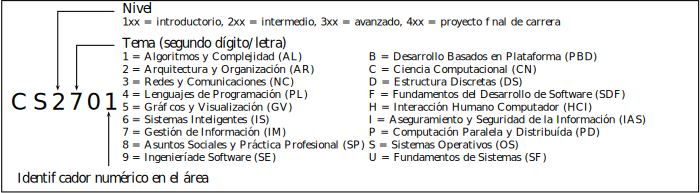
\includegraphics[width=13cm]{\OutputFigsDir/course-coding}
      \caption{Esquema de codificación para los cursos.}\label{fig:course-coding}
      \end{figure}
\end{latexonly}
\begin{htmlonly}
      \begin{rawhtml}
            <p>
                  <img src="./figs/course-coding.png" style="width: 13cm; height: 5cm;">
            </p>
      \end{rawhtml}
\end{htmlonly}

El tipo de curso esta determinado por sus 2 primeras letras. Los posibles códigos para estos tipos son:
\input{\OutputTexDir/prefix-description-ES}

Al mismo tiempo, y de acuerdo a la ley universitaria vigente, los cursos están clasificados en:
\begin{inparadesc}
\item [AF:] Área formativa,
\item [AE:] Área de especialidad,
\item [AB:] Área básica,
\item [AC:] Área complementaria.
\end{inparadesc}

% Table of courses by semesters
\input{\InTexDir/CoursesBySemesters}

\begin{landscape}
\input{\InTexDir/topics-by-course}
\input{\InTexDir/outcomes-by-course}

\section{Malla curricular}\label{sec:vision-grafica}
\vspace{-0.3cm}
Este documento también puede ser analizado desde el punto de vista 
de los prerequisitos de forma gráfica.

\begin{latexonly}
      \begin{figure}[H]
            \includegraphics[width=23cm]{\OutputFigsDir/small-graph-curricula-ES.ps}
            \label{fig:malla-curricular}
            \caption{Malla curricular \SchoolFullName}
      \end{figure}
\end{latexonly}
\begin{htmlonly}
      \begin{rawhtml}
            <div class="center">
                  <iframe scrolling="no" frameborder="0" src="./figs/big-graph-curricula-<LANG_PREFIX>.svg" width="1916pt" height="1218pt">
                  <p><b>This browser is not able to show SVG: try Firefox, Chrome, Safari, or Opera instead.</b></p>
                  </iframe>
            </div>
      \end{rawhtml}
\end{htmlonly}

\end{landscape}

\input{\InTexDir/courses-by-outcome}

\section{Distribución de cursos en la carrera}
\input{\InTexDir/distribution-of-courses} %Graphics by level, by area, etc

\section{Compatibilidad de la carrera con relación a estandares internacionales}
En esta sección presentamos la distribución de cursos por áreas de concentración en 
contraste con las propuestas internacionales de las carreras de la \textit{Computing Curricula} 
de \htmladdnormallink{IEEE-CS}{http://www.computer.org}/\htmladdnormallink{ACM}{http://www.acm.org}.

Es necesario notar que \underline{en algunos casos las materias podrí­an aparecen en más de un eje} 
pues tienen contenido de más de una área. 
Por ejemplo, la materia de sistemas operativos contiene unidades de aplicación 
que pueden ser clasificadas en Tecnologí­a de Información pero al mismo tiempo contiene fundamentos 
de como está estructurado un Sistema Operativo que es del eje de Ciencia de la Computación. 
En estos casos el creditaje ha sido divido entre los ejes correspondientes.
\input{\OutputTexDir/list-of-courses-per-area}

Considerando esta distribución, las figuras~\ref{fig:comparing-curves-\currentarea-\currentinstitution-with-CE} 
a la~\ref{fig:comparing-curves-\currentarea-\currentinstitution-with-SE} 
nos permiten tener una visión gráfica de esta malla curricular frente a las propuestas de 
carreras presentadas por \htmladdnormallink{IEEE-CS}{http://www.computer.org}/\htmladdnormallink{ACM}{http://www.acm.org} en la \textit{Computing Curricula}
\input{\OutputTexDir/comparing-with-standards-\LANG}

%%%%%%%%%%%%%%%%%%%%%%%%%%%%%%%%%%%%%%%%%%%%%%%%%%%%%%%%%%%%%%%%%%%%%%%%%%%%%%%

\begin{btSect}[apalike]{curricula-main}
\section*{\BibliographySection}
\btPrintCited
\end{btSect}
\end{btUnit}
  
\chapter{Contenido detallado por curso}\label{chap:syllabi}
\input{\OutputTexDir/list-of-syllabi}

\OnlyUCSP{\input{\InTexDir/equivalence}}
 
\input{\InTexDir/Laboratories}

\OnlySPC{\input{\InTexDir/professors-and-courses}}
\OnlyMINEDU{\input{\InTexDir/professors-and-courses}}

\OnlySPC{\chapter{Resultados específicos por curso}\label{sec:specific-outcomes-by-course}
%\input{\OutputTexDir/list-of-courses-by-specific-outcome-\LANG}
\begin{landscape}
\input{\OutputTexDir/table-of-courses-by-specific-outcome-\LANG}
\end{landscape}
}

\OnlyMINEDU{\chapter{Resultados específicos por curso}\label{sec:specific-outcomes-by-course}
%\input{\OutputTexDir/list-of-courses-by-specific-outcome-\LANG}
\begin{landscape}
\input{\OutputTexDir/table-of-courses-by-specific-outcome-\LANG}
\end{landscape}
}
